%
% This is a borrowed LaTeX template file for lecture notes for CS267,
% Applications of Parallel Computing, UCBerkeley EECS Department.
% Now being used for CMU's 10725 Fall 2012 Optimization course
% taught by Geoff Gordon and Ryan Tibshirani.  When preparing 
% LaTeX notes for this class, please use this template.
%
% To familiarize yourself with this template, the body contains
% some examples of its use.  Look them over.  Then you can
% run LaTeX on this file.  After you have LaTeXed this file then
% you can look over the result either by printing it out with
% dvips or using xdvi. "pdflatex template.tex" should also work.
%

\documentclass[a4paper,10pt]{article}
\setlength{\oddsidemargin}{0.25 in}
\setlength{\evensidemargin}{-0.25 in}
\setlength{\topmargin}{-0.6 in}
\setlength{\textwidth}{6.5 in}
\setlength{\textheight}{8.5 in}
\setlength{\headsep}{0.75 in}
\setlength{\parindent}{0 in}
\setlength{\parskip}{0.1 in}

%
% ADD PACKAGES here:
%

\usepackage{amsmath,amsfonts,graphicx,hyperref}
\usepackage{tikz}
\usetikzlibrary{positioning}
\tikzset{main node/.style={circle,fill=blue!20,draw,minimum size=1cm,inner sep=0pt},
            }

%
% The following commands set up the lecnum (lecture number)
% counter and make various numbering schemes work relative
% to the lecture number.
%
\newcounter{lecnum}
\renewcommand{\thepage}{\thelecnum-\arabic{page}}
\renewcommand{\thesection}{\thelecnum.\arabic{section}}
\renewcommand{\theequation}{\thelecnum.\arabic{equation}}
\renewcommand{\thefigure}{\thelecnum.\arabic{figure}}
\renewcommand{\thetable}{\thelecnum.\arabic{table}}

%
% The following macro is used to generate the header.
%
\newcommand{\lecture}[4]{
   \pagestyle{myheadings}
   \thispagestyle{plain}
   \newpage
   \setcounter{lecnum}{#1}
   \setcounter{page}{1}
   \noindent
   \begin{center}
   \framebox{
      \vbox{\vspace{2mm}
    \hbox to 6.28in { {\bf Computer Science Track Core Course, \href{http://ist.ac.at/}{IST Austria}
	\hfill Spring 2016}  }
       \vspace{4mm}
       \hbox to 6.28in {Instructors: Krishnendu Chatterjee, Vladimir Kolmogorov, Krzysztof Pietrzak \hfill}
              \vspace{4mm}
                     \hbox to 6.28in {Teaching Assistants: Bernhard Kragl, Josef Tkadlec, Michal Rolinek \hfill}
                            \vspace{4mm}
       \hbox to 6.28in { {\Large \hfill Lecture #1: #2  \hfill} }
       \vspace{2mm}
       \hbox to 6.28in { {\it Lecturer: #3 \hfill Scribe notes by: #4} }
      \vspace{2mm}}
   }
   \end{center}
   \markboth{Lecture #1: #2}{Lecture #1: #2}

   {\bf Notes}: {
   \begin{itemize}
   \item \it Course webpage is located at \href{https://courses.app.ist.ac.at/index.php?id=133}{ https://courses.app.ist.ac.at/index.php?id=133},
   \item  Lecture notes are hosted on GitHub at \href{https://github.com/bkragl/CS-601_S16}{ https://github.com/bkragl/CS-601\_S16},
   \item \it LaTeX template courtesy of UC Berkeley EECS department and my laziness in creating something from scratch.
   \end{itemize}
   }
   
   \vspace*{4mm}
}
%
% Convention for citations is authors' initials followed by the year.
% For example, to cite a paper by Leighton and Maggs you would type
% \cite{LM89}, and to cite a paper by Strassen you would type \cite{S69}.
% (To avoid bibliography problems, for now we redefine the \cite command.)
% Also commands that create a suitable format for the reference list.
\renewcommand{\cite}[1]{[#1]}
\def\beginrefs{\begin{list}%
        {[\arabic{equation}]}{\usecounter{equation}
         \setlength{\leftmargin}{2.0truecm}\setlength{\labelsep}{0.4truecm}%
         \setlength{\labelwidth}{1.6truecm}}}
\def\endrefs{\end{list}}
\def\bibentry#1{\item[\hbox{[#1]}]}

%Use this command for a figure; it puts a figure in wherever you want it.
%usage: \fig{NUMBER}{SPACE-IN-INCHES}{CAPTION}
\newcommand{\fig}[3]{
			\vspace{#2}
			\begin{center}
			Figure \thelecnum.#1:~#3
			\end{center}
	}
% Use these for theorems, lemmas, proofs, etc.
\newtheorem{theorem}{Theorem}[lecnum]
\newtheorem{lemma}[theorem]{Lemma}
\newtheorem{proposition}[theorem]{Proposition}
\newtheorem{claim}[theorem]{Claim}
\newtheorem{note}[theorem]{Note}
\newtheorem{corollary}[theorem]{Corollary}
\newtheorem{definition}[theorem]{Definition}
\newenvironment{proof}{{\bf Proof:}}{\hfill\rule{2mm}{2mm}}

% **** IF YOU WANT TO DEFINE ADDITIONAL MACROS FOR YOURSELF, PUT THEM HERE:

\newcommand\E{\mathbb{E}}

\begin{document}
%FILL IN THE RIGHT INFO.
%\lecture{**LECTURE-NUMBER**}{**DATE**}{**LECTURER**}{**SCRIBE**}
\lecture{1}{February 29th 2016}{Krishnendu Chatterjee}{Amir Goharshady}

% **** YOUR NOTES GO HERE:

% Some general latex examples and examples making use of the
% macros follow.  
%**** IN GENERAL, BE BRIEF. LONG SCRIBE NOTES, NO MATTER HOW WELL WRITTEN,
%**** ARE NEVER READ BY ANYBODY.

\section{Review of Complexity Classes}

\begin{definition}[Alphabet, Strings, Languages, Complexity Class]

A finite alphabet is a finite non-empty set $\Sigma$. A finite string over $\Sigma$ is a finite sequence of elements in $\Sigma$ and the set of all finite strings over $\Sigma$ is denoted $\Sigma^*$. Any set of finite strings over a finite alphabet is called a language, i.e. each subset $L$ of $\Sigma^*$ is a language. Any set of languages is called a complexity class.
\end{definition}

An example of a language is the set $L = \left\{ (G, s, t) \vert G \text{ is a graph and } s \text{ and } t \text{ are vertices of } G \text{ connected by a path}  \right\}$.
The algorithms we look into focus on decision problems. These are ``yes, no" problems defined as follows:
\begin{definition}[Decision Problem]
Given a language $L$, the algorithmic decision problem for $L$ is to find an algorithm $A$ that gets strings as its input and decides whether the given string is in $L$, more specifically we are looking for an algorithm $A$ such that for each string $x$:
$$A(x) = \left\{\begin{matrix}
1 & x \in L\\ 
0 & x \not \in L 
\end{matrix}\right..$$

When there is no fear of confusion, we do not distinguish between a language and its decision problem.
\end{definition}

We are specifically interested in algorithms that run in polynomial time.

\begin{definition}[Worst-Case Runtime of an Algorithm]
Given an algorithm $A$, its worst-case runtime, $T_A$, is a function of the input length, defined to be the maximum runtime of $A$ over all strings of that length, more formally:
$$T_A(n) = \max_{x \in \Sigma^{n}} T(A, x),$$ where $T(A,x)$ is the execution time of $A$ when given $x$ as its input.
\end{definition}

\begin{definition}[Polytime Algorithm]
An algorithm $A$ is a polytime algorithm if its worst-case runtime $T_A$ is bounded by a polynomial.
\end{definition}

We now review some important complexity classes.
\begin{definition}[P] \label{pdef} A language $L$ is in the complexity class P if there exists a polytime algorithm $A$ that solves its decision problem.

\end{definition}

\begin{definition}[NP and coNP]\label{npdef} A language $L$ is in the complexity class NP if there exist a polynomial $p$ and a polytime algorithm $A$ such that:
$$\forall x \in L ~~ \exists y \in \{0, 1\}^{p(\vert x \vert )} ~~ A(x, y) = 1,$$ and 
$$\forall x \not \in L ~~ \forall y \in \{0, 1\}^{p(\vert x \vert )} ~~ A(x, y) = 0.$$

If $A(x, y) = 1$, then $y$ is said to be a witness for $x$. A language $L$ is in coNP if and only if its complement, $\Sigma^* \setminus L$, is in NP.

\end{definition}

\begin{proposition}
P is a subset of NP.
\end{proposition}
\begin{proof}
If $L \in P$, then there exists a polytime algorithm $A$ that solves its decision problem. The same algorithm can be used as in \ref{npdef} with any arbitrary witness to show that $L$ is in $NP$.
\end{proof}

\section{Probabilistic Complexity Classes}
In the probabilistic computation model the algorithms get as their input a string $x$ and a random input $r \in \{0, 1\}^{p(\vert x \vert)}$ for some polynomial $p$, i.e. length of the random input is bounded by a polynomial in terms of $x$'s length. Moreover $r$ is assumed to be chosen uniformly. The algorithm then has to compute an output, or a decision, based on $x$ and $r$.

\begin{definition}[Probabilistic Polytime]
$A$ is a probabilistic polytime algorithm if:
\begin{itemize}
\item Length of the random part, $r$, is bounded by a polynomial in string $x$'s length, and
\item Worst-case runtime of $A$ is bounded by a polynomial.
\end{itemize}
\end{definition}

We now define several useful probabilistic complexity classes.

\begin{definition}[RP -- Randomized Polynomial] \label{rpdef}
A decision problem $L$ is in RP if there exist a polynomial $p$ and a probabilistic polytime algorithm $A$ such that:
$$\forall x \in L ~~~ Pr[A(x, r) = 1] > \frac{1}{2},$$ and $$\forall x \not \in L ~~~ Pr[A(x, r) = 1] = 0,$$
where the probabilities are calculated over all $r \in \{0, 1\}^{p(\vert x \vert)}$ uniformly.

This intuitively means that the algorithm does rejection correctly, i.e. every $x \not \in L$ is always rejected and accepts correctly with probability more than half.
\end{definition}

\begin{definition}[coRP] 
A decision problem $L$ is in coRP if there exist a polynomial $p$ and a probabilistic polytime algorithm $A$ such that:
$$\forall x \in L ~~~ Pr[A(x, r) = 1] = 1,$$ and $$\forall x \not \in L ~~~ Pr[A(x, r) = 1] < \frac{1}{2},$$
where the probabilities are calculated over all $r \in \{0, 1\}^{p(\vert x \vert)}$ uniformly.

This intuitively means that the algorithm does acceptance correctly, i.e. every $x \in L$ is always accepted and rejects correctly with probability more than half.
\end{definition}

Both RP and coRP account for one-sided error, now we define a complexity class that allows two-sided errors, i.e. in both acceptance and rejection.

\begin{definition}[BPP -- Bounded Probabilistic Polynomial] 
A decision problem $L$ is in BPP if there exist a polynomial $p$ and a probabilistic polytime algorithm $A$ such that:
$$\forall x \in L ~~~ Pr[A(x, r) = 1] \geq \frac{2}{3},$$ and $$\forall x \not \in L ~~~ Pr[A(x, r) = 1] \leq \frac{1}{3},$$
where the probabilities are calculated over all $r \in \{0, 1\}^{p(\vert x \vert)}$ uniformly.
\end{definition}

\textbf{Note:} The $\frac{1}{2}$'s in definitions of RP and coRP are arbitrary numbers and one can get same complexity classes using other constant numbers or even constants raised to the power of a polynomial by simply repeating the algorithms. On the other hand in the definition of BPP, the first constant must be bigger than a half and the second one must be less than a half. To see why, consider a coin-tossing algorithm.

\begin{definition}[Extended Decision Algorithms]
An extended decision algorithm $A$ is an algorithm that can return one of the three values $0$, $1$ and $?$, signifying rejection, acceptance and doubt or failure respectively.
\end{definition}

\begin{definition}[ZPP -- Zero-error Probabilistic Polynomial]\label{zppdef}
A decision problem $L$ is in ZPP if there is a polynomial $p$ and a polytime extended algorithm $A$ such that:
$$\forall x ~~ Pr[A(x, r) = ?] \leq \frac{1}{2},$$ and
$$\forall x ~~ \forall r \in \{0, 1\}^{p(\vert x \vert)}  ~~ A(x, r)\neq ? \Rightarrow A(x, r) = \left\{\begin{matrix}
1 & x \in L\\ 
0 & x \not \in L
\end{matrix}\right.,$$
where the probabilities are calculated over all $r \in \{0, 1\}^{p(\vert x \vert)}$ uniformly.

Intuitively, this means that the algorithm fails (is unsure) with probability less than half, and when it does not fail it will always produce the correct answer.
\end{definition}

\begin{proposition}
$P \subseteq RP.$
\end{proposition}
\begin{proof}
Use the algorithm $A$ from \ref{pdef} in \ref{rpdef} and ignore $r$. 
\end{proof}

One can similarly and easily show that $P \subseteq coRP$ and $P \subseteq ZPP$.

\begin{proposition}
$RP \subseteq NP$.
\end{proposition}
\begin{proof}
If $L \in RP$, then for each $x \in L$, $Pr[A(x, r) = 1] > \frac{1}{2}$. Since this probability is positive, there exists an $r$ such that $A(x, r) = 1$. This $r$ can be used as a witness for $x$. Similarly, if $x \not \in L$, no witness can be found since $Pr[A(x, r) = 1] = 0$.
\end{proof}

\textbf{Note:} We do not know whether $P=RP$ or whether $RP=NP$. 

\begin{proposition}
$RP \subseteq BPP.$
\end{proposition}
\begin{proof}
Let $L \in RP$. Take an algorithm $A$ for it as in \ref{rpdef} and construct the algorithm $A^{(k)}$ which takes a string $x$ as input and works as follows:
\begin{tabbing}
\hspace*{.25in} \= \hspace*{.25in} \= \hspace*{.25in} \= \hspace*{.25in} \= \hspace*{.25in} \=\kill
\> Choose random strings $r_1, r_2, \ldots, r_k$\\
\>{\bf if} $\exists i ~~ A(x, r_i) = 1$ {\bf then } \\
\>\> {\bf return} 1 \\
\>{\bf else} \\
\>\> {\bf return} 0\\
\>{\bf endif} 
\end{tabbing}

If $x \in L$, then $A(x, r)$ returns 1 with probability more than $\frac{1}{2}$, so $A^{(k)}$ returns 1 with probability more than $1 - \frac{1}{2^k}$. It is sufficient to choose $k$ such that this value gets bigger than $\frac{2}{3}$. On the other hand, if $x \not \in L$, then $A(x, r)$ always returns 0 and so does $A^{(k)}$.

\end{proof}

\textbf{Note:} The relationship between BPP and NP is an open problem.

\textbf{Homework:} Prove that if $NP \subseteq BPP$, then $NP = RP$.

$$\begin{tikzpicture}
    \node[main node] (1) {$NP$};
    \node[main node] (2) [right =1.5cm of 1]  {$BPP$};
    \node[main node] (3) [right =1.5cm of 2]  {$coNP$};
    \node[main node] (4) [below = 1.5cm of 1] {$RP$};
    \node[main node] (5) [below = 1.5cm of 3] {$coRP$};
    \node[main node] (6) [below = 3cm of 2] {$P$};

    \path[draw,thick]
    (6) edge node {} (4)
    (6) edge node {} (5)
    (4) edge node {} (1)
    (4) edge node {} (2)
    (5) edge node {} (2)
    (5) edge node {} (3)
    ;
    %%
\end{tikzpicture}$$
The figure above shows relations between various complexity classes. An edge between two classes means that the upper class is a superset of the lower one.

\begin{definition}[Probabilistic Average Runtime]
Given a probabilistic algorithm $A$, its average runtime is a function of the length, $n$, of input $x$ defined as:
$$\max_{x \in \{0, 1\}^n} E[T(A, x, r)],$$
where $T(A, x, r)$ is the runtime of $A$ with inputs $x$ and $r$ and the expectation is defined uniformly over all possible $r$. Intuitively, for each input $x$, we take the average time the algorithm requires to terminate on $x$ among all random $r$'s and then we take the maximum over all strings $x$ of the fixed length $n$.  
\end{definition}
\begin{definition}[ACP -- Average Case Polynomial]\label{acpdef}
A decision problem $L$ is in ACP if there is an algorithm $A$ with polynomial average runtime that always produces the right answer for $L$.
\end{definition}

\begin{proposition}
$ZPP = ACP.$
\end{proposition}
\begin{proof}
We first prove that $ZPP \subseteq ACP$. Let $L \in ZPP$ and $A$ be an algorithm as in \ref{zppdef}. We provide the following algorithm $A'$:
\begin{tabbing}
\hspace*{.25in} \= \hspace*{.25in} \= \hspace*{.25in} \= \hspace*{.25in} \= \hspace*{.25in} \=\kill
\> 1: Choose a random string $r$\\
\>{\bf if} $A(x, r) \not = ?$ {\bf then } \\
\>\> {\bf return} $A(x, r)$ \\
\>{\bf else} \\
\>\> {\bf goto} 1\\
\>{\bf endif} 
\end{tabbing}

This algorithm, will always return the correct answer upon termination. Assuming that $A(x, r)$ terminates in time at most $t$, $A'$, when run on $x$, has an average runtime of at most $$t + \frac{1}{2} t + \frac{1}{4} t + \ldots = t \sum_{i=0}^\infty \frac{1}{2^i} = 2t.$$

Now we prove that $ACP \subseteq ZPP$. Let $A$ be an algorithm as in \ref{acpdef}. We create the following algorithm $A'$:

\begin{tabbing}
\hspace*{.25in} \= \hspace*{.25in} \= \hspace*{.25in} \= \hspace*{.25in} \= \hspace*{.25in} \=\kill
\> Run the first $2 t(x)$ steps of $A(x)$, where $t(x)$ is the average runtime of $A(x)$. \\
\>{\bf if} an answer was returned (a decision was made) {\bf then } \\
\>\> {\bf return} the same answer (decision) \\
\>{\bf else} \\
\>\> {\bf return} ?\\
\>{\bf endif} 
\end{tabbing}

When the returned value is not ?, $A'$ returns only correct answers because $A$ has the same property. We should only show that given a string $x$, the probability that $A'$ returns $?$ is at most $\frac{1}{2}$. Suppose otherwise, then $A(x)$ terminates in $2 t(x)$ steps with probability less than $\frac{1}{2}$ which is a contradiction.

\end{proof}

\end{document}





